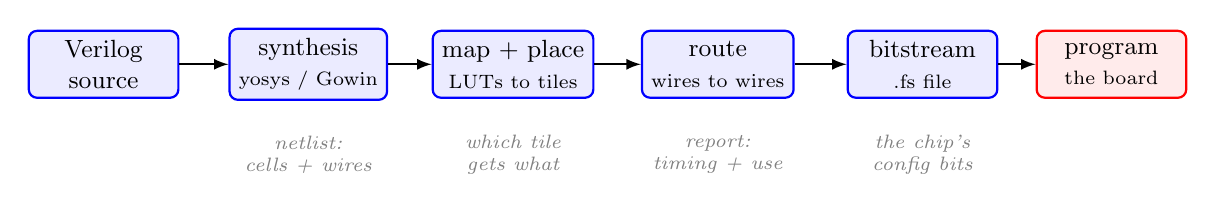
\begin{tikzpicture}[x=1cm,y=1cm, >=latex,
  stage/.style={draw=blue, thick, fill=blue!8, rounded corners=3pt, minimum width=1.9cm, minimum height=0.85cm, font=\small, align=center},
  stagenote/.style={font=\scriptsize\itshape, text=gray, align=center}]
\node[stage] (src) at (0,0) {Verilog\\ source};
\node[stage] (syn) at (2.6,0) {synthesis\\ \scriptsize yosys / Gowin};
\node[stage] (map) at (5.2,0) {map + place\\ \scriptsize LUTs to tiles};
\node[stage] (par) at (7.8,0) {route\\ \scriptsize wires to wires};
\node[stage] (bit) at (10.4,0) {bitstream\\ \scriptsize .fs file};
\node[stage, draw=red, fill=red!8] (bd) at (12.8,0) {program\\ \scriptsize the board};
\foreach \a/\b in {src/syn, syn/map, map/par, par/bit, bit/bd}
  \draw[->, thick] (\a) -- (\b);
\node[stagenote] at (2.6,-1.15) {netlist:\\ cells + wires};
\node[stagenote] at (5.2,-1.15) {which tile\\ gets what};
\node[stagenote] at (7.8,-1.15) {report:\\ timing + use};
\node[stagenote] at (10.4,-1.15) {the chip's\\ config bits};
\end{tikzpicture}
